\documentclass[conference]{IEEEtran}
\usepackage{amsmath}
\usepackage{graphicx}
\usepackage{booktabs,array}
\usepackage{tikz}
\usepackage{pgfplots}
\pgfplotsset{compat=1.17}
\usepackage[hidelinks]{hyperref}
\usepackage{cite}
% ---- Slot for a figure taken from a cited paper -------------------------
% Appears only if the image file exists, so the PDF builds either way.
% #1 file, #2 caption, #3 credit line (e.g. "Reproduced from~\cite{saied2022}, CC BY 4.0.")
\newcommand{\paperfig}[3]{\IfFileExists{#1}{%
  \begin{figure}[t]\centering\includegraphics[width=\columnwidth]{#1}%
  \caption{#2 #3}\end{figure}}{}}
\hypersetup{
  pdftitle={Recent Research Progress in Probabilistic Shaping for Clipping- and Peak-Limited LED Links},
  pdfauthor={Yugeshwaran P (23BEC1404)},
  pdfsubject={BECE306L Digital Communication Systems -- Literature Survey}}

\begin{document}
\title{Probabilistic Shaping for Clipping- and Peak-Limited LED Links: Recent Progress}
\author{\IEEEauthorblockN{Yugeshwaran P (23BEC1404)}
\IEEEauthorblockA{School of Electronics Engineering, VIT \textbullet{} BECE306L Digital Communication Systems -- Literature Survey, 2026--27\\
Topic: Advanced Modulation Formats for High-Speed Digital Communication \textbullet{} yugeshwaran.p2023@vitstudent.ac.in}}
\maketitle


\section{Introduction}
Visible light communication (VLC) and short-reach optical interconnects use intensity modulation with direct detection (IM/DD): the signal must be real and non-negative, and the LED or modulator is linear only over a limited current range. Multicarrier formats handle the frequency-selective LED response well, but their high peak-to-average power ratio (PAPR) forces clipping. Recent work adapts probabilistic constellation shaping (PCS) to such clipping- and peak-limited links. The chosen base paper~\cite{pham2026} optimizes PCS for clipped DC-biased optical OFDM (DCO-OFDM). This survey reviews 26 journal papers from 2021--2026; Fig.~\ref{fig:concept} illustrates the problem they address.

\begin{figure}[t]\centering
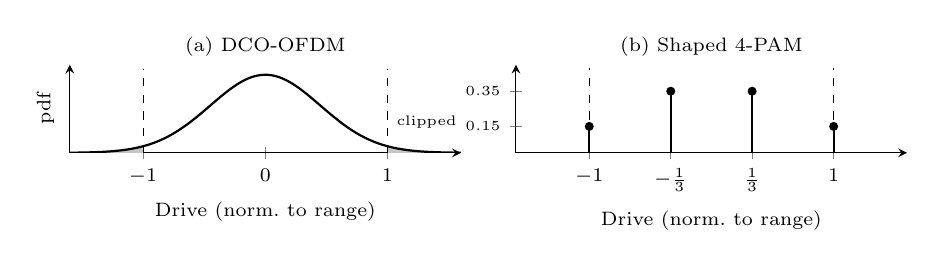
\begin{tikzpicture}[declare function={g(\x)=exp(-(\x)^2/(2*0.45^2))/(0.45*sqrt(2*pi));}]
\begin{axis}[name=A,width=0.54\columnwidth,height=2.7cm,xmin=-1.6,xmax=1.6,ymin=0,ymax=1.0,
  axis lines=left,xtick={-1,0,1},ytick=\empty,ylabel={pdf},
  xlabel={Drive (norm.\ to range)},label style={font=\scriptsize},tick label style={font=\scriptsize},
  title={(a) DCO-OFDM},title style={font=\scriptsize,yshift=-1.5ex}]
\addplot[draw=none,fill=gray!45,domain=1:1.6,samples=30]{g(x)}\closedcycle;
\addplot[draw=none,fill=gray!45,domain=-1.6:-1,samples=30]{g(x)}\closedcycle;
\addplot[black,thick,domain=-1.6:1.6,samples=120]{g(x)};
\draw[dashed](axis cs:-1,0)--(axis cs:-1,0.95);\draw[dashed](axis cs:1,0)--(axis cs:1,0.95);
\node[font=\tiny,align=center] at (axis cs:1.32,0.35){clipped};
\end{axis}
\begin{axis}[at={(A.east)},anchor=west,xshift=7mm,width=0.54\columnwidth,height=2.7cm,xmin=-1.6,xmax=1.6,ymin=0,ymax=0.5,
  axis lines=left,xtick={-1,-0.333,0.333,1},xticklabels={$-1$,$-\frac13$,$\frac13$,$1$},ytick={0.15,0.35},yticklabel style={font=\tiny},
  xlabel={Drive (norm.\ to range)},label style={font=\scriptsize},tick label style={font=\scriptsize},
  title={(b) Shaped 4-PAM},title style={font=\scriptsize,yshift=-1.5ex}]
\addplot[ycomb,black,thick,mark=*,mark size=1.2pt] coordinates{(-1,0.15)(-0.333,0.35)(0.333,0.35)(1,0.15)};
\draw[dashed](axis cs:-1,0)--(axis cs:-1,0.48);\draw[dashed](axis cs:1,0)--(axis cs:1,0.48);
\end{axis}
\end{tikzpicture}
\caption{The two constraint models (illustration drawn for this survey; dashed: LED range). (a) The near-Gaussian DCO-OFDM signal is clipped. (b) A PAM constellation fits the range, so shaping acts on the peak.}\label{fig:concept}
\end{figure}

\section{Optical OFDM and the Clipping Problem}
Zhang \emph{et al.}~\cite{zhang2021} survey the evolution of optical OFDM for both VLC and fiber, and position layered ACO-OFDM between ACO- and DCO-OFDM in the trade-off between spectral and power efficiency. Bai and Hranilovic~\cite{bai2021} propose a layered antisymmetry-constructed clipped OFDM that needs less than half of the multiplications and additions of layered ACO-OFDM. Pham and Ishihara~\cite{pham2026} show that PCS can increase the PAPR of DCO-OFDM and thus the clipping distortion; they formulate capacity maximization with clipping, which is non-convex, and solve it sub-optimally by projected gradient descent with a single shaping distribution for all subcarriers. Alrakah \emph{et al.}~\cite{alrakah2024} analyse clipping noise in OFDM-based VLC and show that DCO-OFDM with PAPR reduction achieves a lower BER than conventional DCO-OFDM.

An alternative is to avoid the Gaussian-like OFDM waveform. Hussin and Shalaby~\cite{hussin2021} compare DFT-spread OFDM with OFDM for an indoor single-LED link in terms of BER and PAPR. Saied, Li and Rabie~\cite{saied2022} propose DFT-spread optical PAM, which in simulation has about 7\,dB lower PAPR than DCO-OFDM and in experiment needs about 2.5\,dB less average transmit power. For vehicular VLC, Saied \emph{et al.}~\cite{saied2023} report a 9\,dB PAPR advantage of DFT-spread PAM, but find that DCO-OFDM is better when the signal bandwidth greatly exceeds the LED modulation bandwidth.


% Third-party figure slot 1: from [5] Saied, Li, Rabie, IEEE Access 2022 (verify CC BY licence first)
\paperfig{figures/third_party/fig_ref5.png}{TODO: describe what the figure shows (e.g.\ PAPR of DFT-spread PAM vs.\ DCO-OFDM).}{Reproduced from~\cite{saied2022}, CC BY 4.0.}

\section{Shaping Under Peak Constraints}
Without optical amplification, an IM/DD link is limited by peak rather than average power. Wiegart \emph{et al.}~\cite{wiegart2021} optimize the input distribution of 4-PAM under the peak constraint set by the modulator's extinction ratio, and confirm gains in reach and rate adaptability experimentally. Che, Cho and Chen~\cite{che2021} show that a peak-constrained system can be partly or fully converted into an average-constrained one, where conventional PCS helps, if the transmitter DSP raises the PAPR; they verify this with 4- and 8-PAM. Che and Chen find that faster-than-Nyquist PAM-4 gains over higher-order formats on gradually decaying channels~\cite{che2022}, and review IM-DD modulation and DSP beyond 200\,Gb/s~\cite{che2024}. Liang and Kahn~\cite{liang2025a} use a high-rate continuous approximation to obtain closed-form capacity-achieving inputs and shaping gains for optical channels, including direct detection; Liang \emph{et al.}~\cite{liang2025b} add peak and average power constraints and note that PS must expand the peak-to-average ratio, which complicates peak-limited systems.

In VLC, Gutema \emph{et al.}~\cite{gutema2022} demonstrate a three-LED WDM link with probabilistically shaped OFDM at 10.81\,Gb/s, 25\,\% above adaptive bit-and-power loading. Nguyen \emph{et al.}~\cite{nguyen2025} jointly optimize the PAM symbol probabilities and the precoder of a multi-user VLC broadcast channel under amplitude constraints, with sum-rate gains of about 17.5\,\% (8-PAM) and 19.2\,\% (16-PAM) over uniform signaling. Pham and Ishihara~\cite{pham2025} use PCS of $M$-PAM for physical-layer security in VLC and obtain a design that meets the BER requirement over the whole optical power range, where uniform signaling does not. Gao \emph{et al.}~\cite{gao2025} design multidimensional geometrically shaped constellations for MISO VLC under per-LED optical power constraints at finite blocklength.

\begin{table}[t]\centering\footnotesize\setlength{\tabcolsep}{3pt}
\caption{Representative works and their constraint model}\label{tab:sum}
\begin{tabular}{@{}lll>{\raggedright\arraybackslash}p{3.0cm}@{}}\toprule
Ref. & Waveform & Constraint & Main contribution \\\midrule
\cite{pham2026} & DCO-OFDM & Clipping & PCS via PGD \\
\cite{saied2022} & DFT-s PAM & LED range & 7\,dB lower PAPR \\
\cite{alrakah2024} & DCO-OFDM & Clipping & PAPR reduction, BER \\
\cite{nguyen2025} & PAM & Amplitude & PCS + precoding \\
\cite{liang2025b} & DD, PAM & Peak + avg. & Shaping gains \\
\cite{gao2025} & MISO VLC & Per-LED power & Multidimensional GS \\\bottomrule
\end{tabular}\end{table}

\section{Practical Shaping and Distribution Matching}
Short distribution matchers make PCS implementable. Chen \emph{et al.}~\cite{chen2022} optimize enumerative sphere shaping, beating constant-composition matching at short blocklengths. Matsumine \emph{et al.}~\cite{matsumine2021} realize probabilistic amplitude shaping with short linear block codes and report 0.3--1.0\,dB shaping gain for blocks shorter than 24 symbols. For multicarrier links, Liu \emph{et al.}~\cite{liu2022} flatten the uneven subcarrier SNR with partial Walsh--Hadamard precoding, cutting the real multiplications from $2P^2-2P$ to $2P\log_2P$ with about 1\,dB sensitivity gain over conventional PS. Autoencoder-learned constellations are more robust to channel uncertainty than QAM~\cite{jovanovic2022}. In OFDM sensing and communication (ISAC), Geiger \emph{et al.}~\cite{geiger2026} compare geometric, probabilistic and joint shaping and Du \emph{et al.}~\cite{du2026} extend PCS to mismatched-filter sensing; Guo \emph{et al.}~\cite{guo2026} reach 101.47\,b/s/Hz with PS-16QAM over 7-core 3-mode fiber.

% Third-party figure slot 2: from Alrakah et al., Photonics 2024 (verify CC BY licence first)
\paperfig{figures/third_party/fig_alrakah2024.png}{TODO: describe what the figure shows.}{Reproduced from~\cite{alrakah2024}, CC BY 4.0.}

\section{LED Nonlinearity}
Inside its range, the LED is also nonlinear. Deng \emph{et al.}~\cite{deng2022} build a physics-based LED model and a low-complexity post-compensator implemented in real time on an FPGA, and Park \emph{et al.}~\cite{park2022} compensate LED nonlinearity in DCO-OFDM VLC with coefficient-approximation predistortion and a bidirectional LSTM.

\section{Open Questions and Conclusion}
Three trends emerge: shaping is moving to peak- and amplitude-constrained models~\cite{wiegart2021,che2021,nguyen2025,liang2025b,gao2025}; DFT-spread waveforms are reconsidered for LEDs for their lower PAPR~\cite{saied2022,saied2023}; and short matchers and learned shaping make PCS practical~\cite{chen2022,matsumine2021,jovanovic2022}. Two questions remain open in the reviewed papers. First, OFDM shaping under clipping~\cite{pham2026} uses one distribution for all subcarriers and does not load shapes and powers jointly with the clipping operating point. Second, peak-constrained PAM shaping has not been compared directly with an optimized clipped DCO-OFDM link of the same bandwidth and LED range.

\makeatletter\def\IEEEbibitemsep{0pt plus .5pt}\makeatother
\bibliographystyle{IEEEtran}
{\scriptsize\bibliography{refs}}
\end{document}
